\section{Applied 2015: Solution \footnote{Lucas Janson, Gene Katsevich, Kenneth Tay, Stephen Bates, Nikos Ignatiadis, Isaac Gibbs, Dan Kluger and M.H.}}


\subsection*{Problem 1: Exponential family manipulations for the Gamma distribution}
\begin{itemize}
\item[(a)] \begin{align*}
g(x) &= \exp \left\{ (v-1)\log(x) - x/\lambda - v\log(\lambda) - \log(\Gamma(v)) \right\} I(x > 0)\\
&= \exp \left\{ \begin{pmatrix} v-1 \\ 1/\lambda \end{pmatrix}^\top \begin{pmatrix}\log x \\ -x \end{pmatrix} - \left[v\log(\lambda) + \log(\Gamma(v)) \right] \right\}I(x > 0),
\end{align*}

so $\eta = \begin{pmatrix} v-1 \\ 1/\lambda \end{pmatrix}$, $y = \begin{pmatrix}\log x \\ -x \end{pmatrix}$, and $\psi = v\log(\lambda) + \log(\Gamma(v))$.

\item[(b)] Since $\log x $ is the sufficient statistic for $\eta_1 = v - 1$, we can compute its expectation by differentiating the log partition function:
\begin{equation*} \mathbb E_{v, \lambda}[\log(x)] = \frac{d}{d(v-1)}\psi(v, \lambda) = \frac{d}{dv}(\psi(v, \lambda)) = \log \lambda + \frac{\Gamma'(v)}{\Gamma(v)}. \end{equation*}
\end{itemize}


% Problem 2
\subsection*{Problem 2: Bias in cross-validation, \citep[Ch. 7.10]{hastie2009elements}}

\paragraph{Context:} As you have seen, this type of question comes up a lot. A good reference to read is Chapter 7.10 of the Elements of Statistical Learning \citep*{hastie2009elements}. Also Exercise 7.10 therein could be instructive.

\begin{itemize}
\item[(a)] No, it will be biased upwards. This is because the models trained in CV use just $9/10$'s of the training data, and so will (in general) have a larger error rate than if all the training data was used. The CV estimate would be unbiased for $\hat{C}(x)$'s error if you had $9/10$ as much training data \textbf{and} you also average over the given training data. In particular, we do not expect the CV estimate to be unbiased for the prediction error of the classifier training on the given training data, but rather to be unbiased for the average prediction error averaged over the observed training data (see section 7.12 in \citep*{hastie2009elements} and \citep*{Bates2022CrossVal}).  

\item[(b)] For any binary classifier $\hat{C}_{\text{any}}$, whether or not it was trained on all the data or any particular subset of the data, $$\mathbb P[\hat C_{\text{any}}(X) \neq Y] = \mathbb E[ \mathbb E  [I \{ \hat C_{\text{any}}(X) \neq Y \} |X]] = \mathbb E[1/2] = 1/2.$$

Thus the error rate of $\hat{C}$ is $1/2$. The CV estimate will now be unbiased, since that error rate is the same for all classifiers and in particular does not depend on how much training data there is or which subset of the data was used.

\item[(c)] Yes, it will bias the CV estimate downwards. You should add the screening into the procedure so that it is performed within each CV fold. Doing selection on the entire data set introduces dependencies between folds. Thus, the CV estimate will be too optimistic.
\end{itemize}


% Problem 3
\subsection*{Problem 3:  Confidence intervals for an exponential}
First-order accuracy means that the coverage error of the confidence interval decreases at order $O(1/\sqrt{n})$. Second-order accuracy means that it decreases at order $O(1/n)$.

\begin{itemize}
\item[(a)] Note that $y$ has gamma distribution with shape parameter $1$ and scale parameter $\lambda$. Hence, $\mathbb E[y] = \lambda = SD(y)$. The MLE is $\bar{y}$ (the mean), so $\bar{y} \pm z_{.975}\bar{y}/\sqrt{n}$ is an asymptotically-valid 95\% confidence ($z_{.975}$ is the $0.975$th quantile of the standard Gaussian).

\textbf{Remark:} The above is a bit of a shortcut though that leverages a CLT for the mean of IID variables, but since it would be a good idea to practice constructing confidence intervals based on the asymptotic theory of the MLE in an exponential family I also present the calculations using that approach below. \newline

To construct confidence intervals for the MLE note that the log-likelihood is 

$$l(\lambda) = -n \bar{y}/\lambda -n \log (\lambda).$$

Taking derivatives and setting the log likelihood to zero it is easy to check that $\hat{\lambda}=\bar{y}$ gives the MLE and further $$\ddot{l}(\lambda)=-\frac{2n \bar{y}}{\lambda^3} + \frac{n}{\lambda^2}.$$

Thus the observed Fisher information is $-\ddot{l}(\hat{\lambda})=n/\bar{y}^2$, so $(\hat{\lambda} -\lambda) \stackrel{\cdot}{\sim} N(0,[n/\bar{y}^2]^{-1} )$.  Recalling, $\hat{\lambda}=\bar{y}$ this gives the confidence interval $\bar{y} \pm z_{.975}\bar{y}/\sqrt{n}$.

%One could also probably use the empirical SD instead of $\bar{y}$ for the width, but I'm not sure I'd consider that quite as ``standard'' when you know the exact distribution.

\item[(b)] Using shape-scale parametrization: $y \sim \text{Gam}(1, \lambda)$ implies $2y/ \lambda \sim \text{Gam}(1, 2) = \chi_2^2$. Summing up over the $y_i$, we obtain $2n\bar{y}/\lambda \sim \chi^2_{2n}$, so an exact 95\% CI is \[\left[
		\frac{2n\bar{y}}{\chi^2_{2n,.975}},\frac{2n\bar{y}}{\chi^2_{2n,.025}}\right],\]
		where $\chi^2_{2n,\alpha}$ is the $\alpha$th quantile of the
		$\chi^2_{2n}$ distribution.

\item[(c)] \textbf{(Out of curriculum.)} We could use the BCa (``bias-corrected and accelerated") method. Details can be found in Section 11.4 of \citep*{efron2016computer}.

\item[(d)] \textbf{(Out of curriculum.)} I think the ABC bootstrap is what the question is going for. It needs only 1\% as much computation as the BCa method. (See \citep*{DiCiccioBootstrap} for details.)

\end{itemize}


\subsection*{Problem 4: Causal inferences based on structural assumptions}
\paragraph{Context:} \citet*{mooij2016distinguishing}

First, let us assume that the data is not truncated, i.e. this is a full sample from the joint distribution of $(x, y)$. Then, it is possible that $x$ causes $y$, since $y$ appears to be a smooth function of $x$ plus symmetrically distributed noise of constant variance. However, $y$ definitely cannot cause $x$, since the variance of $x|y$ jumps at the point $y_0$ when the smooth curve mapping $y \mapsto x$ becomes a one-to-many function. 

Now, it is conceivable that we have only received a truncated data set, and that, for example, the domain of $x$ might extend further to the right. However, it is still difficult to imagine a way the data can be extrapolated to allow $x$ to be a smooth function of $y$ plus symmetrically distributed, constant variance noise.

% Problem 5
\subsection*{Problem 5: Huber loss connection with $L_1$ penalization}


\paragraph{Context:} This problem is quite nice as it combines ideas from convex optimization and robust statistics and appears to be from~\citet{she2011outlier}. Note this is a good example of why you should read the entire question. Doing part (d) first can help with part (b).


\begin{itemize}
\item[(a)] The idea is to allow a few (the $\ell_1$ penalty induces sparsity in ${\bf \gamma}$) data points to be corrupted while still basically minimizing squared error. Each $\gamma_i$ represents how much of an outlier the corresponding $y_i$ is, with $\gamma_i=0$ interpreted as saying that $y_i$ is not an outlier at all.

\item[(b)] First of all, note that the problem is convex, so we are in good shape. Next, note that for any fixed $\beta$, the optimization problem decouples over the vector ${\gamma}$. Specifically, define,
\[r_i = y_i - x_i^\top \beta\]
so that $r_i$ is the $i$th residual. Then, as a function of $\gamma$, our loss function is,
\begin{align*}
	\ell({\gamma})&=\frac{1}{2}\sum_{i=1}^n(r_i-\gamma_i)^2 + \lambda \sum_{i=1}^N |\gamma_i | \\
	&=\sum_{i=1}^N \left(\frac{1}{2}(r_i-\gamma_i)^2 +\lambda |\gamma_i|\right). 
\end{align*}
The value, ${\gamma}^*$ that minimizes the above loss function is given by
\begin{align*}
	\gamma_i^* &=\argmin_{\gamma_i} \frac{1}{2}(r-i-\gamma_i)^2+\lambda|\gamma_i|\\
	&=\begin{cases}
		r_i + \lambda  &\text{if } r_i < -\lambda,\\
		0 & \text{if } -\lambda \le r_i \le \lambda,\\
		r_i - \lambda  & \text{if } r_i > \lambda.
	\end{cases}\\
	&=S(r_i;\lambda)
\end{align*}
That is, $\gamma_i^*$ is the \emph{soft-threshold function} of $r_i$. Furthermore, if ${\gamma}$ is fixed, then our model is a simple linear regression problem with response $Y-{\gamma}$. This suggests the following iterative block descent algorithm,
\begin{enumerate}
	\item[1.] Start with $\hat{\gamma}^0 = 0$.
	\item[2.] For $t=0,1,\ldots,$
	\begin{enumerate}
		\item Set $\hat{\beta}^t = (X^\top X)^{-1}X^\top(Y-\hat{\gamma}^t)$.
		\item Set $r^t = Y - X\hat{\beta}^t$ and $\hat{\gamma}^{t+1} = S(r^t;\lambda)$.
	\end{enumerate}
\end{enumerate}
So one way to solve the optimization problem is with the above iterative algorithm. Another approach is to use part (d) and show that the given optimization problem is equivalent to minimizing the Huber loss. A third approach would be to recast the problem as a (partial) LASSO problem with design matrix $\widetilde{X} = [X,I_N] \in \reals^{N \times (p+N)}$, parameters $\widetilde{\beta}=(\beta,{\gamma}) \in \reals^{p + N}$ and an $L^1$ penalty on $\gamma$. For optimization details see here  See \url{https://www.stat.cmu.edu/~ryantibs/convexopt-F18/lectures/coord-desc.pdf} and \url{https://scs.hosted.panopto.com/Panopto/Pages/Viewer.aspx?id=03b0a4f5-734f-4f91-974b-a9910130191e}.
\item[(c)] We can apply cross-validation with the criterion being just the residual sum of squares:
\begin{equation*}
\sum_{i \in \text{out-of-fold}} \left( y_i - \sum_{j=1}^p x_{ij}\hat{\beta}_j \right)^2.
\end{equation*}
There is one problem with this. Certain out-of-fold data points may be outliers. So it might make sense to use a different loss function to evaluate the errors on such points. One possibility would be to use the Huber loss in cross-validation instead of squared error loss.

Alternatively, if you have prior information about the frequency of outliers, you may just adjust $\lambda$ to achieve a pre-specified level of sparsity in ${\bf \gamma}$.
	
\item[(d)] 	From part (b) we know that for a fixed $\beta$, the optimal $\gamma^*$ is given by
\[\gamma^*_i = S(r_i;\lambda), \]
where $r_i = y_i - x_i^\top \beta$ and $S(r;\lambda)$ is the soft-threshold function defined above. If $|r_i| \le \lambda$, then $\gamma_i^* = 0$ and 
\begin{align*}
	\frac{1}{2}(r_i-\gamma_i^*)^2 + \lambda |\gamma_i^*| = \frac{1}{2}r_i^2 = \rho(r_i;\lambda),
\end{align*}
where $\rho(\cdot;\lambda)$ is the Huber loss function from the question. Furthermore, if $|r_i| >\lambda$, then $S(r_i;\lambda) = r_i - \mathrm{sign}(r_i)\lambda$ and 
\[|\gamma_i| = |r_i - \mathrm{sign}(r_i)\lambda| = |r_i|-\lambda. \]
Thus,
\begin{align*}
	\frac{1}{2}(r_i-\gamma_i^*)^2 + \lambda |\gamma_i^*| &= \frac{1}{2}(\mathrm{sign}(r_i)\lambda)^2 +\lambda(|r_i|-\lambda) \\
	&=\lambda|r_i|-\frac{1}{2}\lambda^2\\
	&=\rho(r_i;\lambda).
\end{align*}
Thus, with the optimal $\gamma^*$, the original objective function can be written as
\begin{align*}
	\frac{1}{2}\sum_{i=1}^n (y_i-x_i^\top \beta-\gamma_i^*)^2 + \lambda\sum_{i=1}^n |\gamma_i^*|\\
	&=\sum_{i=1}^n \rho(y_i-x_i^\top \beta;\lambda),
\end{align*}
showing that the two problems have the same $\beta$ solution.
	
\item[(e)]  Criterion (1) can help, but there are likely scenarios where it does not succeed in removing the influence of the far away data point. Let's consider the problem with a fixed $\lambda$ (i.e. outlier budget). If we have a point whose feature vector is far away from the data, then the straight line fit through the rest of the points might be very far away from the outlying data point (for example this can happen if the true response function is nonlinear but is quite linear locally). Hence, while adding the extra $\gamma$ term will help, there might not be enough outlier budget to correct for this data point entirely, so the fit through the rest of the data might still be impacted. Moreover, the criterion (1) devotes just as much outlier budget to low leverage outliers as it does to high leverage outliers. Note that larger values of $\lambda$ correspond to smaller outlier budgets.  

A different approach would be to use clustering to identify any outliers (e.g. $k$-means clustering, and identify points with largest distance to their cluster centroid as outliers). We can then either investigate/remove them or give them lower weight in the optimization. Note that if we only use the $x$ values for $k$-means then this approach is unsupervised.
\end{itemize}



% Problem 6
\subsection*{Problem 6: Life tables, survival curves and GLMs}

\paragraph{Context:} \citet{efron2016computer} Chapter 9
\begin{itemize}
\item[(a)] We first review a commonly used approach to estimate the probability that a client survives past each age: the Kaplan-Meier estimator.
Let $T$ denote the (random) survival time. Let $p_j = \mathbb P[T < j+1|T \geq j]$ be the probability of dying before reaching age $j+1$ conditional on reaching age $j$. Then, the survival function (conditional on reaching age 60) is 
\begin{equation*} s_i = \mathbb P[T \geq i|T \geq 60] = \prod_{j = 60}^{i-1} \mathbb P[T \geq j+1|T \geq j] = \prod_{j = 60}^{i-1} (1-p_j).
\end{equation*}

Now, let $d_j$ be the number of deaths at age $j$ and $n_j$ the number of people still alive at age $j$. We can estimate $\hat p_j = d_j/n_j$
\begin{equation} 
\hat s_i = \prod_{j = 60}^{i-1} (1-\hat p_j) = \prod_{j = 60}^{i-1} \left(1-\frac{d_j}{n_j}\right).
\label{eq:KaplanMeyerEst}
\end{equation}
This estimator is the Kaplan--Meier estimator

The question is asking us how the actuary computed the survival curve. While the Kaplan--Meier estimator is a natural guess, we should also point out that based on the table this is indeed what the actuary did: the column titled ``proportion" has the values of  $\hat p_i = d_i/n_i$, and the column titled ``Survival" has the entries $\hat s_{i+1}$, given by \eqref{eq:KaplanMeyerEst}.

\item[(b)] We could use logistic regression to model $\text{logit}(p_j)$ quadratically in age:
\[d_j \overset{\text{ind}}\sim \text{Bin}(n_j, p_j), \quad \log\left(\frac{p_j}{1-p_j}\right) = \beta_0 + j\beta_1 + j^2\beta_2.\]

Once we get the estimated $\hat{p}_j$, we can use them in the same survival formula as in part (a): 
\[s^{\text{quad}}_i = \prod_{j=60}^{i-1}(1-\hat{p}_j).\]

To implement this in R, one could use the glm function. In particular, suppose each of the first three columns in the table is stored as a vector in R.
\begin{lstlisting}
ageSquared <- age^2
quadFit <- glm(cbind(deaths,number-deaths) ~ age+ageSquared, 
			   family = binomial)
SurvQuad <- cumprod(1-quadFit$fitted.values)
\end{lstlisting}

Unfortunately, you will not be able to double check on the exam that this is what the second actuary did to compute the column titled SurvQuad, because you will not have access to R. That being said, this is a reasonable guess based on the problem description and the fact that this actuary has training in GLMs and computed a ``quadratically smoothed curve". 
\end{itemize}

\textbf{Aside:} If you are curious whether the answer to part (b) is the answer that the author of the Quals question was going for, it was indeed the answer the author had in mind. In particular the procedure in part (b) recovers the entries in the column tiled SurvQuad. See the below screenshot for verification of this:

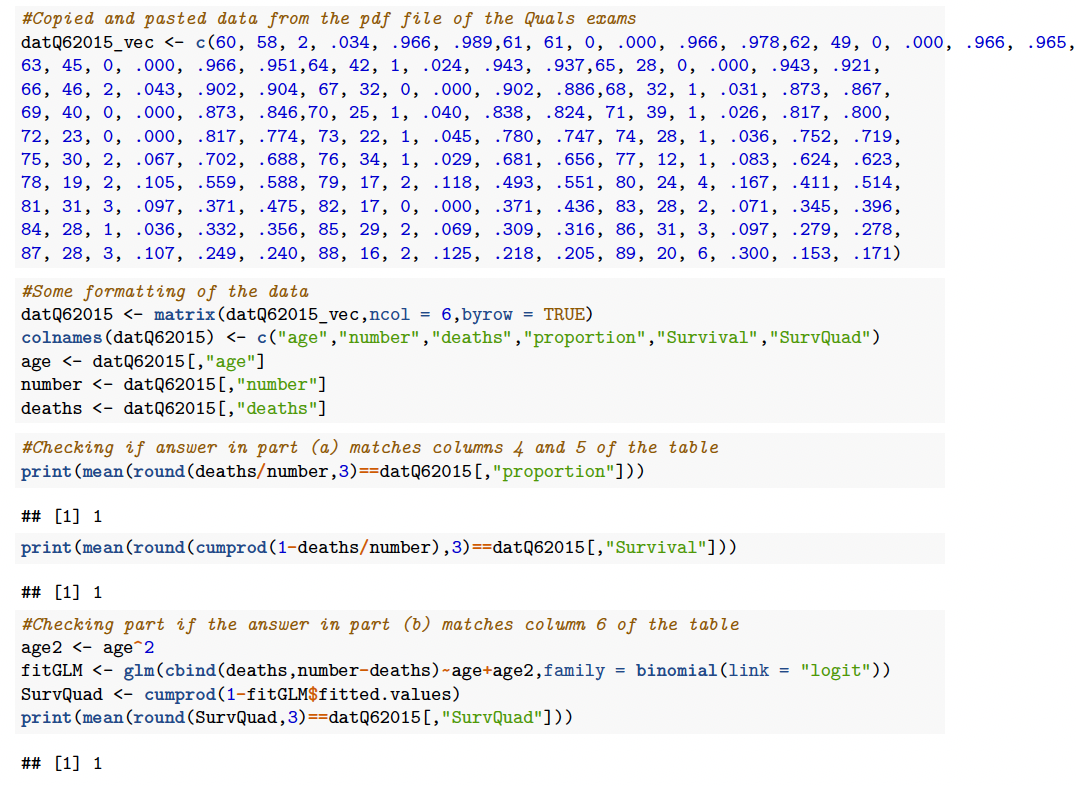
\includegraphics[width = \textwidth]{Q62015SanityCheck.png}


